\documentclass[10pt,a4paper]{article}
\usepackage[utf8]{inputenc}
\usepackage{standalone}
\usepackage{amsmath,amsfonts,amssymb, float}
\usepackage{import, amstext}
\usepackage{graphicx}
\usepackage{hyperref}
\usepackage{titlesec}
%\usepackage[round]{natbib}
\usepackage{rotating,array,float}
\newcolumntype{C}{>{\centering\arraybackslash}X}
\usepackage{booktabs,tabularx,dcolumn,adjustbox}
\usepackage[font=normal,skip=.333\baselineskip]{caption}
\usepackage[margin=2.5cm,headheight=0pt,headsep=0pt]{geometry}
\usepackage[flushleft]{threeparttable}
\titleformat*{\section}{\Large\bfseries}
%\titleformat*{\subsection}{\large\bfseries}
\titleformat*{\subsubsection}{\large\bfseries}
\titleformat*{\paragraph}{\large\bfseries}
\titleformat*{\subparagraph}{\large\bfseries}
\parindent 0px
\usepackage{fullpage, pgfplots}
\usepackage{multicol}
\usepackage{makeidx}
\RequirePackage{chapterbib}
\usepackage{color,soul}
%\usepackage{refcheck}

%\author{
%  Dharmendra Dangi\\
%  \texttt{dangi28dharmendra06@gmail.com}
%  \and
%  Abhay Sharma\\
%  \texttt{abhaysharma01702@gmail.com}
%}
%   \vspace{0.5cm} % Adds some vertical space  
%
\date{}
\title{\textbf{Harnessing CNNs and Embedding Techniques for Enhanced
Sentiment Classification}} 
\usepackage{setspace}



\begin{document}
\spacing{1.2}

\maketitle

\section*{Abstract}

This study evaluates the performance of various embedding techniques combined with Convolutional Neural Networks (CNNs) for sentiment analysis on two datasets: Amazon product reviews and IMDB movie reviews. Specifically, we assess three embedding approaches: GloVe, FastText, and Word2Vec.
Our experiments reveal that the CNN + FastText configuration achieved the highest accuracy of 97.29\% on the IMDB dataset, demonstrating its effectiveness in capturing semantic nuances through subword information. In contrast, the CNN + Word2Vec approach consistently underperformed, particularly on the Amazon dataset, with an accuracy of 92.06\%. GloVe showed competitive results, in IMDB sentiment analysis, achieving an accuracy of 96.78\%. The findings indicate that embedding choice significantly impacts model performance, highlighting the potential of FastText in sentiment analysis tasks.\\
Keywords - FastText, Sentiment Analysis, CNN, Word2Vec, GloVe
\\[8pt]

\begin{multicols}{2}
\section*{Introduction}

Sentiment analysis, a technique used to interpret and classify users' thoughts, feelings, and opinions expressed in text, has become essential in understanding customer feedback and improving business processes. According to Mariusz\cite{Michalowski_2024} with over 2.5 exabytes of data generated daily, extracting meaningful insights from this vast pool of information is crucial for businesses. Sentiment analysis helps organizations monitor and analyze public opinions, user reviews, and social media posts, categorizing sentiments into positive, negative, or neutral classes. These insights guide decisions regarding product development, marketing strategies, and customer service, thus enhancing customer engagement and satisfaction.

In recent years, advancements in machine learning (ML) and natural language processing (NLP) have led to more accurate sentiment analysis methods, surpassing traditional lexicon-based techniques. One such advancement is the use of deep learning models, particularly Convolutional Neural Networks (CNNs), which have proven effective in capturing local features within text. CNNs' ability to extract hierarchical patterns from sequential data makes them a powerful tool for text classification tasks, including sentiment analysis.

\hl{This study aims to explore the effectiveness of different word embedding techniques—specifically GloVe, FastText, and Word2Vec—when integrated with CNNs for sentiment analysis. Word embeddings are crucial in transforming words into numerical representations, enabling models to capture semantic relationships between words. By comparing these embeddings, this research investigates how they influence the performance of CNNs in sentiment classification tasks using two datasets: IMDB movie reviews}\cite{N_2019} \hl{and Amazon fine food reviews}\cite{Project_2017}.


\section*{Related Works}

\hl{The origins of sentiment analysis can be traced back to early approaches that relied on lexicon-based methods. These methods used predefined dictionaries with annotated sentiment scores for words or phrases. One of the contributions in this field was the development of the Valence Aware Dictionary and sEntiment Reasoner (VADER) by Hutto and Gilbert}\cite{hutto2014vader}. \hl{VADER was designed to evaluate sentiment in social media text and is known for its ability to capture both intensity and polarity of sentiments. However, one major limitation of lexicon-based approaches is their inability to understand nuanced language features, such as sarcasm, negations, or domain-specific terms.}

\hl{With the rise of machine learning, more sophisticated techniques emerged, including supervised learning models that automatically learn patterns in data. Early studies on machine learning-based sentiment analysis explored methods like Support Vector Machines (SVMs)}\cite{wang2024word2vec} \hl{and Logistic Regression (LR)}\cite{ghosh2022sentiment}. \hl{However, these models heavily relied on feature engineering and were less effective in capturing the complex semantic relationships between words.}

\hl{The introduction of deep learning models, especially Recurrent Neural Networks (RNNs) and Long Short-Term Memory (LSTM) networks, marked a significant advancement. Murthy et al.}\cite{murthy2020text} \hl{employed LSTM-based models for sentiment analysis of IMDB movie reviews and demonstrated superior performance over traditional machine learning methods. Nandwani and Verma}\cite{nandwani2021review} \hl{also concluded that neural network-based models outperform traditional approaches.} 

\hl{Recently, word embeddings have emerged as a critical component of sentiment analysis models. These embeddings, such as Word2Vec, GloVe, and FastText, represent words in dense vector spaces, enabling models to understand semantic relationships between words beyond simple frequency counts. Word2Vec, introduced by Mikolov et al.}\cite{mikolov2013efficient}\hl{, utilizes neural networks to create vector representations for words based on their context within a corpus. GloVe (Global Vectors for Word Representation), developed by Pennington et al.}\cite{pennington2014glove}\hl{, improves upon Word2Vec by considering word co-occurrence statistics, which enhances the embeddings' ability to capture global relationships. FastText, an extension of Word2Vec, models subword information, making it more robust in handling out-of-vocabulary words and morphological variations}\cite{bojanowski2017enriching}.

\hl{Neural networks, particularly CNNs, have gained popularity for sentiment analysis due to their ability to automatically extract features from raw text. Kim}\cite{kim2014convolutional} \hl{demonstrated the use of CNNs for sentence classification and highlighted their efficiency in detecting local patterns, such as sentiment cues in specific phrases or words. }

\section*{Methodology}
\hl{This section outlines the step-by-step approach used to develop, train, and evaluate the model.}


\subsection*{Datasets}
\hl{This paper utilizes two datasets for analysis. The first is the }\href{https://www.kaggle.com/datasets/lakshmi25npathi/imdb-dataset-of-50k-movie-reviews}{\hl{IMDB Movie Reviews Dataset}}\cite{N_2019}, \hl{which consists of 50,000 movie reviews. The second is the} \href{https://www.kaggle.com/datasets/snap/amazon-fine-food-reviews}{\hl{Amazon Reviews Dataset} }\cite{Project_2017}\hl{, containing 568,454 product reviews. These datasets provide a diverse range of opinions and feedback, making them ideal for evaluating sentiment analysis models.}

\subsection*{\hl{Data Preprocessing}}
\hl{Textual data requires extensive preprocessing to prepare it for model input. The process begins with text cleaning, where stopwords and irrelevant elements like special characters, URLs, and emojis are removed, and the text is standardized by converting all characters to lowercase. Next, the text is tokenized into individual words. Lemmatization follows, reducing words to their base forms. Sentences are then padded with zeros to ensure uniform length. Finally, the tokens are transformed into vectors using various word embedding techniques such as Word2Vec, GloVe, and FastText, making the data ready for model input.}
%
%\subsection*{Data Splitting}
%
%The dataset is divided into three subsets: training (70\%), validation (15\%), and test (15\%). To ensure that the distribution of sentiment classes is consistent across all subsets, stratified splitting is employed. Furthermore, to address class imbalance, the majority class is under sampled, ensuring a more balanced representation of sentiment classes in the training data. This approach aims to improve model performance by mitigating the impact of class imbalance while preserving the overall class distribution.



\subsection*{Model Design}
\hl{As shown in figure}\ref{model_fig} \hl{the architecture of the model utilizes Convolutional Neural Networks (CNNs), } 
\end{multicols}
\begin{figure}[H]
\begin{center}
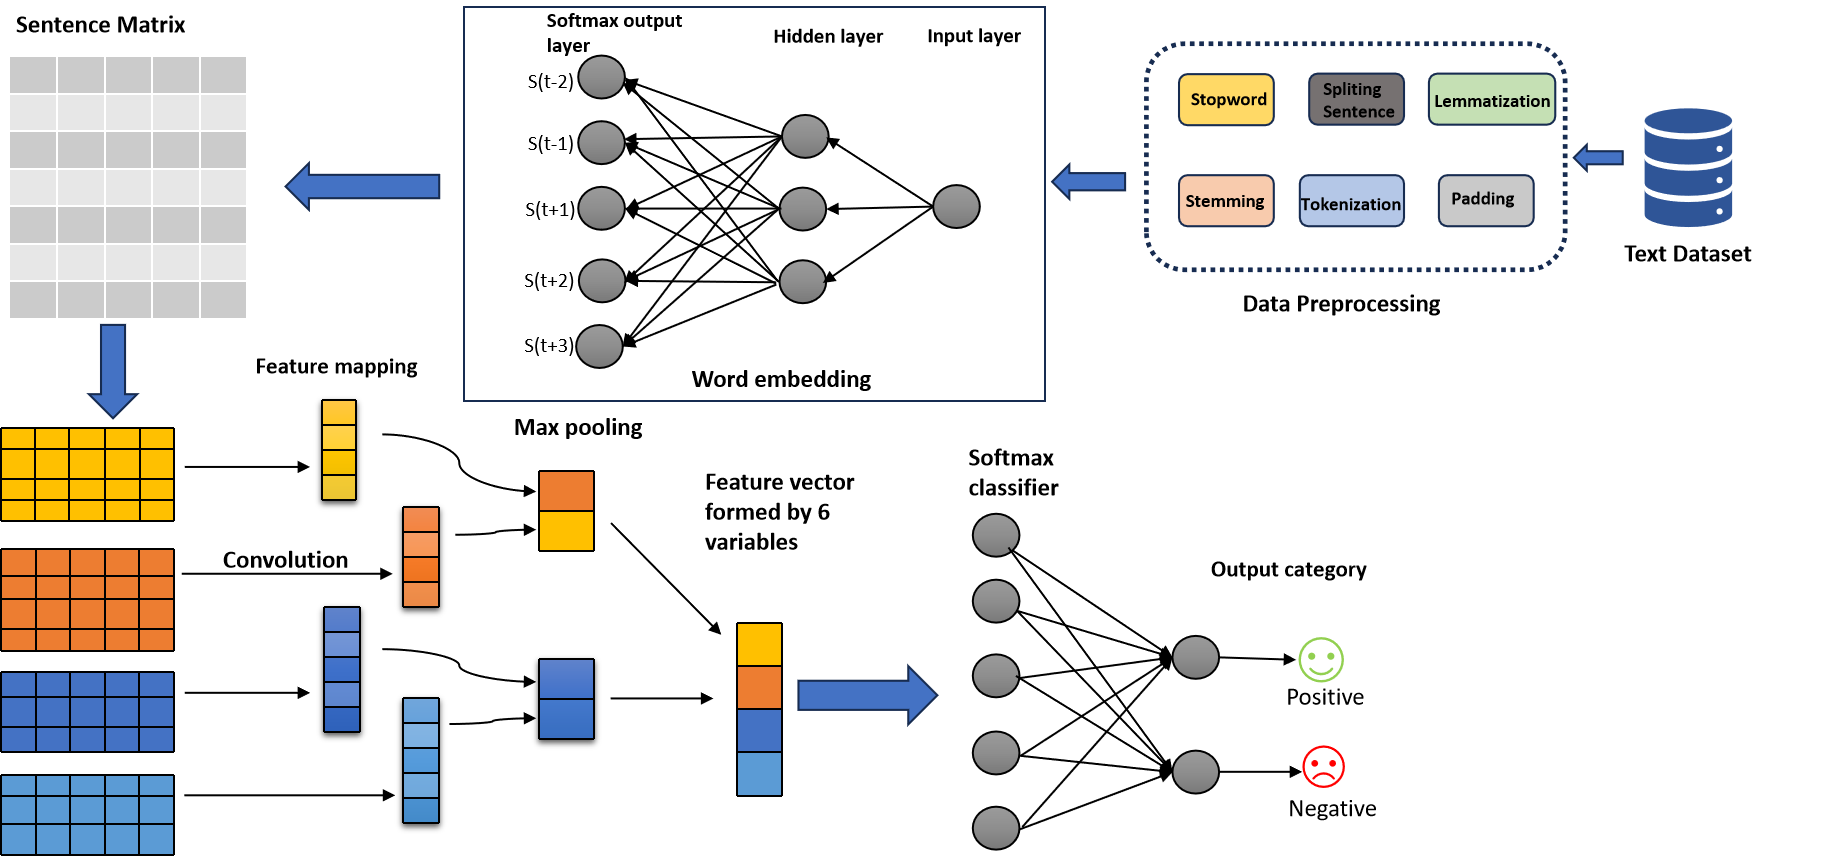
\includegraphics[scale=0.55]{cnn_model}\\
\end{center}
\caption{Architecture of the CNN-based Sentiment Classification Model with Word Embedding Techniques}
\label{model_fig}
\end{figure}
\begin{multicols}{2}

\hl{which are widely recognized for their ability to capture local features in sequential data. CNNs have been effectively used in text classification tasks, such as sentiment analysis, where they are able to detect meaningful patterns in sequences of words }\cite{kim2014convolutional}\cite{zhang2015character}.

\hl{The architecture of our model consists of several key layers. It begins with an input layer that accepts word vectors, which are then passed to a convolutional layer with ReLU activation. This layer performs a convolution operation using filters to detect local features within the input sequences, generating a feature map. The output of the convolution layer is subsequently fed into a max pooling layer, which reduces the spatial dimensions of the feature map while retaining the most important features. This approach to feature extraction has been widely used in the literature for improving performance on text classification tasks}\cite{conneau2017supervised}.\\
\hl{After passing through multiple convolution and max pooling layers with varying filter sizes, the resulting features are flattened into a one-dimensional vector. This vector is then passed to a fully connected (dense) layer, which combines the features extracted from the convolution and pooling layers to make the final sentiment prediction.}\\
\hl{The output from the dense layer is passed to the output layer. For the IMDB dataset, the output layer uses a sigmoid activation function, while for the Amazon Reviews dataset, a softmax activation function is used to handle multi-class classification.}


\subsection*{\hl{Hyperparameter Tuning}}
\hl{To optimize model performance, several hyperparameters were tuned using Bayesian optimization, a technique that leverages probabilistic models to make informed decisions and efficiently search the hyperparameter space.}

\subsection*{Model Compilation and Training}
\hl{
Once the model architecture was defined, we compiled it using the Adam optimizer, known for its efficiency with large datasets. For the loss function, binary crossentropy was used for the IMDB dataset, given its binary classification nature, while categorical crossentropy was applied to the Amazon dataset, as it deals with multi-class classification. The evaluation metric for both datasets was accuracy, to assess the model's performance in predicting sentiment correctly.

The model was trained using the training subset of the dataset, and early stopping was employed to avoid overfitting, monitoring the validation loss. We also utilized dropout regularization to further prevent overfitting and ensure that the model generalizes well.}\\



\subsection*{Model Evaluation}
\hl{To evaluate the performance of the model, we implemented a comprehensive framework. The datasets were split into training (70\%), validation (15\%), and test (15\%) subsets, using stratified sampling to maintain the class distribution. We also applied k-fold cross-validation to assess the model's generalization across different data subsets. The evaluation metrics included accuracy, precision, recall, and F1-score, providing a balanced measure of the model’s ability to classify sentiment. A confusion matrix was used to identify misclassifications. To reduce the risk of overfitting, we employed techniques such as early stopping, dropout regularization, and undersampling to address class imbalance. This evaluation strategy allowed us to thoroughly analyze the model’s performance, highlighting its strengths and areas for further improvement.}



\section*{Result}
This study emphasizes the critical role that word embedding techniques play in enhancing sentiment analysis performance when integrated with Convolutional Neural Networks (CNNs). Among the evaluated configurations, the CNN + FastText model achieved outstanding results, attaining 97.29\% accuracy on the IMDB dataset. This demonstrates its ability to capture nuanced semantic information through subword-level embeddings. GloVe also showed strong performance, with 96.78\% accuracy, while Word2Vec lagged behind, achieving only 92.06\% accuracy on the Amazon dataset.\\
These results underscore the significant impact of embedding choice on model performance, with FastText emerging as the most effective solution for sentiment analysis tasks across diverse and complex datasets. Additionally, when compared to established baselines such as Logistic Regression, SVM, LSTM, and GRU, the CNN + FastText model consistently outperformed these methods, reaffirming its superior capability to capture semantic nuances, as shown in Table \ref{results}.


\begin{threeparttable}[H] 
\caption{Accuracy Comparison with established baseline models}
\begin{tabularx}{.5\textwidth}{@{} l *{3}{C} @{}} 
\toprule
\textbf{Dataset} &\textbf{Approach} & \textbf{Accuracy(\%)}\\
\midrule
&SVM+Word2Vec\cite{wang2024word2vec} & 84.78  \\ \addlinespace
&LSTM+Word2Vec\cite{akinmadenlp} & 93.00  \\ \addlinespace
Amazon&\textbf{CNN+Word2Vec} & 92.06  \\ \addlinespace
& \textbf{CNN+GloVe} & 93.55 \\ \addlinespace
 & \textbf{CNN+FastText}  & 93.79 \\ \addlinespace


&&  \\ \addlinespace

 & GRU+Word2Vec\cite{pandit2024regular} &  86.82 \\ \addlinespace
& LR+TF-IDF\cite{ghosh2022sentiment} &  90.30 \\ \addlinespace
IMDB& MLP+Lexicon\cite{shaukat2020sentiment} &  91.90 \\ \addlinespace
&\textbf{CNN+GloVe} & 96.78 \\ \addlinespace
& \textbf{CNN+Word2Vec} & 96.78  \\ \addlinespace
& \textbf{CNN+FastText}  & 97.29 \\ \addlinespace
\bottomrule
\end{tabularx}

\label{results}
\end{threeparttable}
% \vspace{1pt}


\section*{Conclusion}
\hl{This study demonstrates the importance of word embedding techniques in enhancing sentiment analysis with Convolutional Neural Networks (CNNs). The CNN + FastText model achieved the best performance and outperformed traditional baselines like Logistic Regression, SVM, LSTM, and GRU, reaffirming its robustness.\\
Despite these successes, challenges persist. Analysis showed that the models had difficulty handling ambiguous or sarcastic sentiments, especially in the IMDB dataset, highlighting limitations in detecting subtle linguistic cues. \\
Future work will focus on incorporating advanced techniques, such as attention mechanisms, to enhance the model’s ability to interpret nuanced and ambiguous sentiments, addressing the challenges identified during error analysis. These improvements aim to refine the model’s capacity to handle subtle linguistic cues, ensuring greater accuracy and robustness. }



\section*{Statements and Declarations}
\subsubsection*{Competing Interests}
The authors declare that there is no conflict of interest.
\subsubsection*{Data Availability}
The authors confirm that the data supporting the findings of this study are available within the article
\end{multicols}

%\section*{Acknowledgement}
%
%\subsection*{CRediT Author Statement}
%
%Dr. Dharmendra Dangi: Conceptualization, Methodology, Validation, Resources, Supervision, Administration.\\
%Abhay Sharma: Methodology, Software, Formal Analysis, Investigation, Resources, Visualization, Writing - Review \& Editing.
%\subsection*{Conflict of Interest} 
%The authors declare that they have no conflict of interest.
%\subsection*{Ethical Approval}
%No human participants or animals were involved in any of the studies conducted by the authors for this article.
%
%\subsection*{Informed Consent} Not applicable.
%\subsection*{Funding} This research did not receive any specific grant from funding agencies in the public, commercial, or not-for-profit sectors.
%\subsection*{Declaration of Interest} The authors declare that they have no financial or personal relationships that could inappropriately influence or bias the content of this paper.


%\nocite{*}
\newpage
\bibliographystyle{plain}
\bibliography{references}




\end{document}




